Since the blockchain technology is proposed, different methods for visualization and analysis are explored. As Bitcoin is the first and main blockchain network in the world and the data can be accessed publicly, much literature conducts researches based on it. Generally, there are three categories of related works for the visualization of a blockchain system.
\begin{itemize}
    \item \textbf{Visualization of Blockchain Information} \\
        There are a lot of online visualization applications which can visualize the static information of transactions and blocks on a blockchain system. They display the information in detail and usually serve as the base for analysis.
    \item \textbf{Analysis of Bitcoin Transactions} \\
        As Bitcoin becomes a popular peer-to-peer network recently, most of the recent literature focuses on the analysis of the relationships between transactions and blocks on Bitcoin network. They try to recognize special patterns to gain economic experience and prevent criminal activities.
    \item \textbf{Analysis of Consensus Protocols} \\
        An analysis of the consensus protocols on the blockchain networks is an interesting topic as it can reveal the potential applications on blockchain platforms.
\end{itemize}

% TODO: deep analyze the visualization

\section{Visualization of Blockchain Information}

There are some online tools and applications that provide visualization of the static status and information of transactions and blocks on Bitcoin network. Tri A. Sundara et al. \cite{Sundara2017} summarized 8 visualization applications and compared their visualization methods and technologies. We shortly review these applications here, so the main difference between our application and them can be identified clearly.
\clearpage

\begin{itemize}
    \item \textbf{Bitbonkers} \cite{bitbonkers} \\
        Bitbonkers rendered a live 3D animation of transactions and blocks. Balls represent transactions, and they keep dropping down to the plate from the top. On the other hand, cubics represent blocks. The sizes of balls are different according to their total values. (Figure \ref{fig:bitbonkers})
        \begin{figure}[htb]
            \centering
            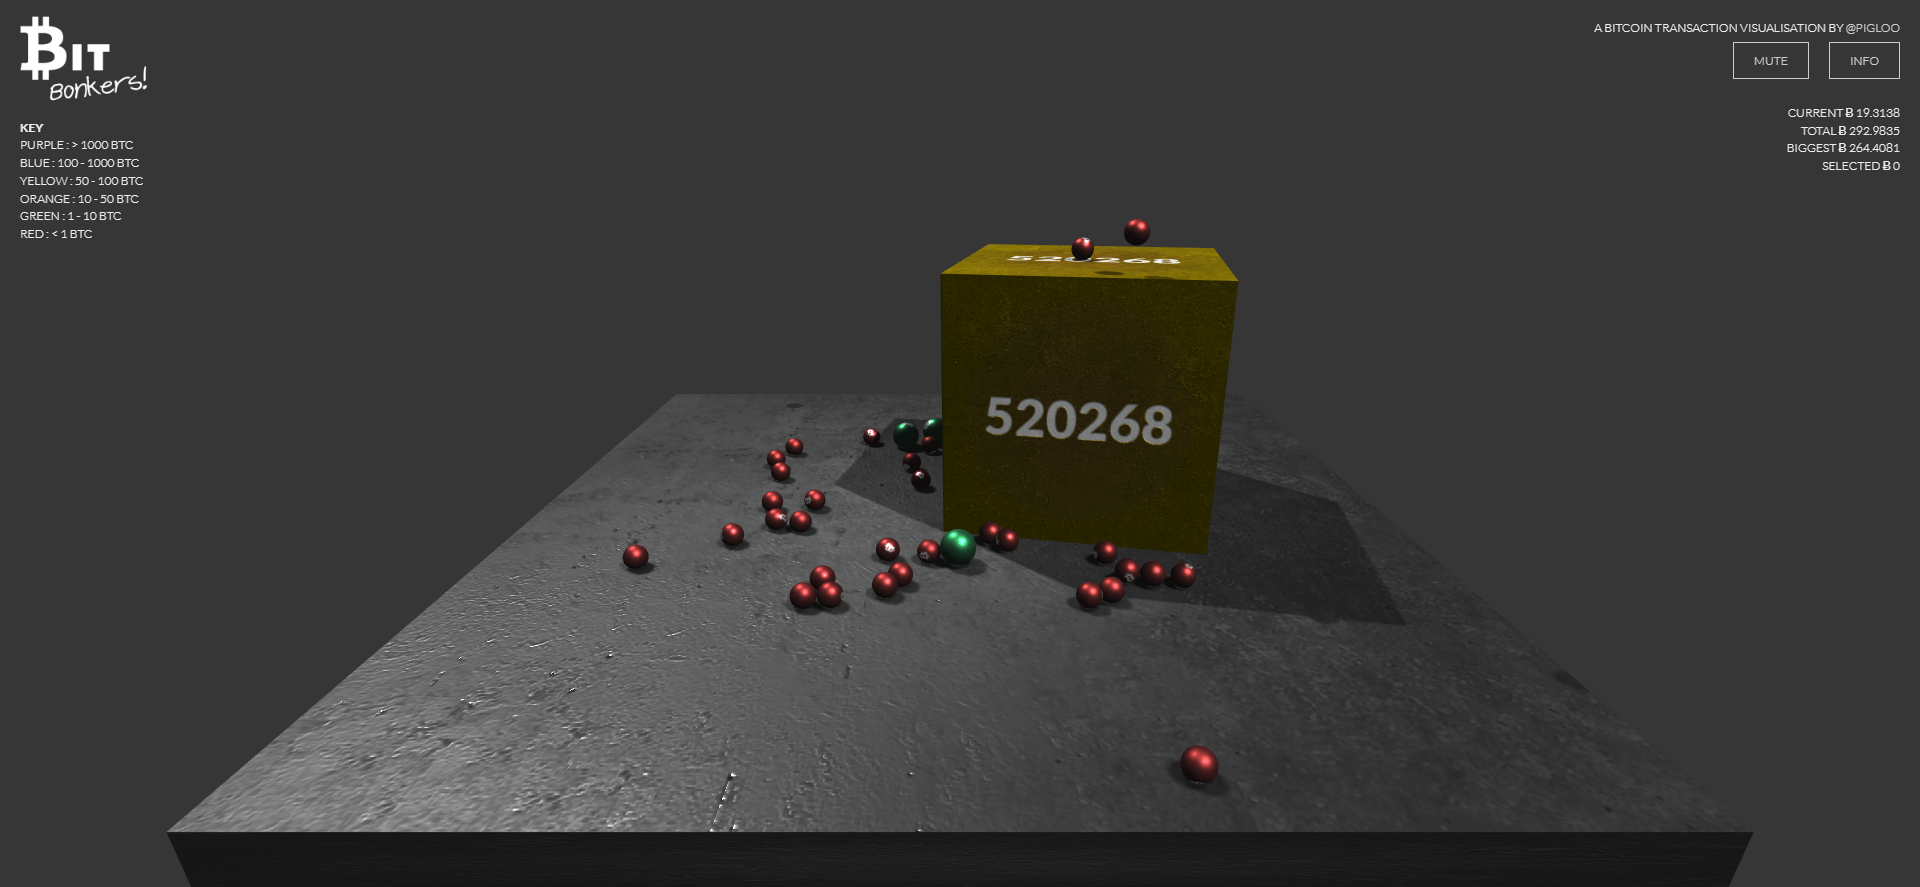
\includegraphics[width=\textwidth]{related_bitbonkers}
            \caption{Bitbonkers.}
            \label{fig:bitbonkers}
        \end{figure}
    \item \textbf{Bitnodes} \cite{bitnodes} \\
        Bitnodes focused on the visualization of the distribution of nodes on Bitcoin network. The density of nodes can be observed clearly on the world map. (Figure \ref{fig:bitnodes})
        \begin{figure}[htb]
            \centering
            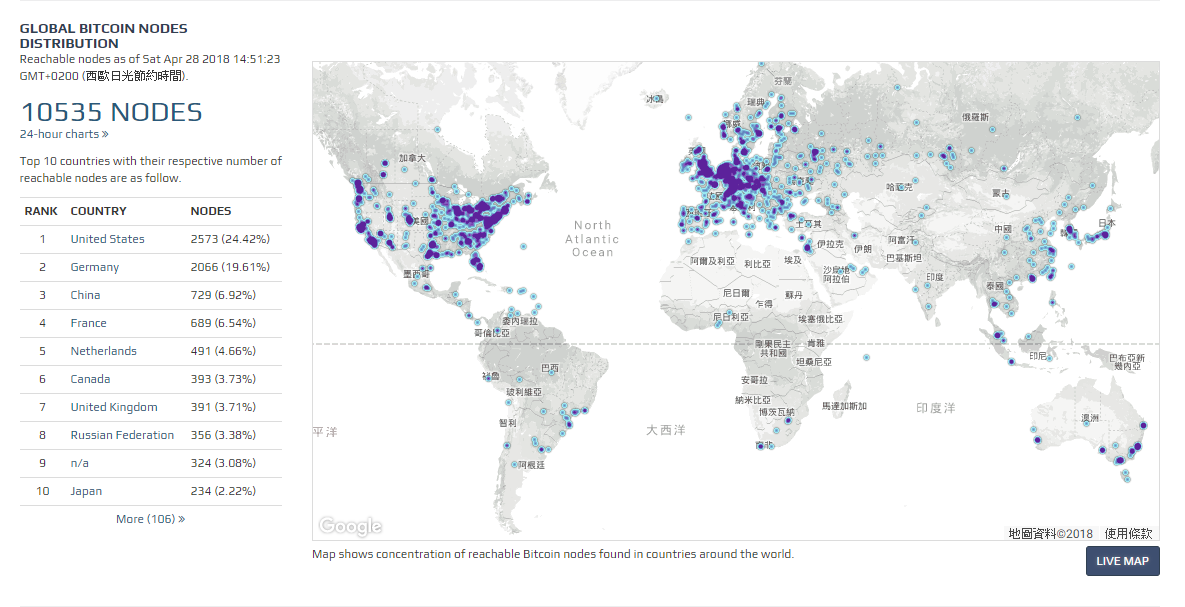
\includegraphics[width=\textwidth]{related_bitnodes}
            \caption{Bitnodes.}
            \label{fig:bitnodes}
        \end{figure}
    \clearpage
    \vspace*{\fill}
    \item \textbf{BitcoinCity} \cite{bitcoincity} \\
        BitcoinCity is a cute visualization of Bitcoin. It used a road to chain the blocks, and the houses with different heights on both sides of the road represented transactions. (Figure \ref{fig:bitcoincity})
        \begin{figure}[htb]
            \centering
            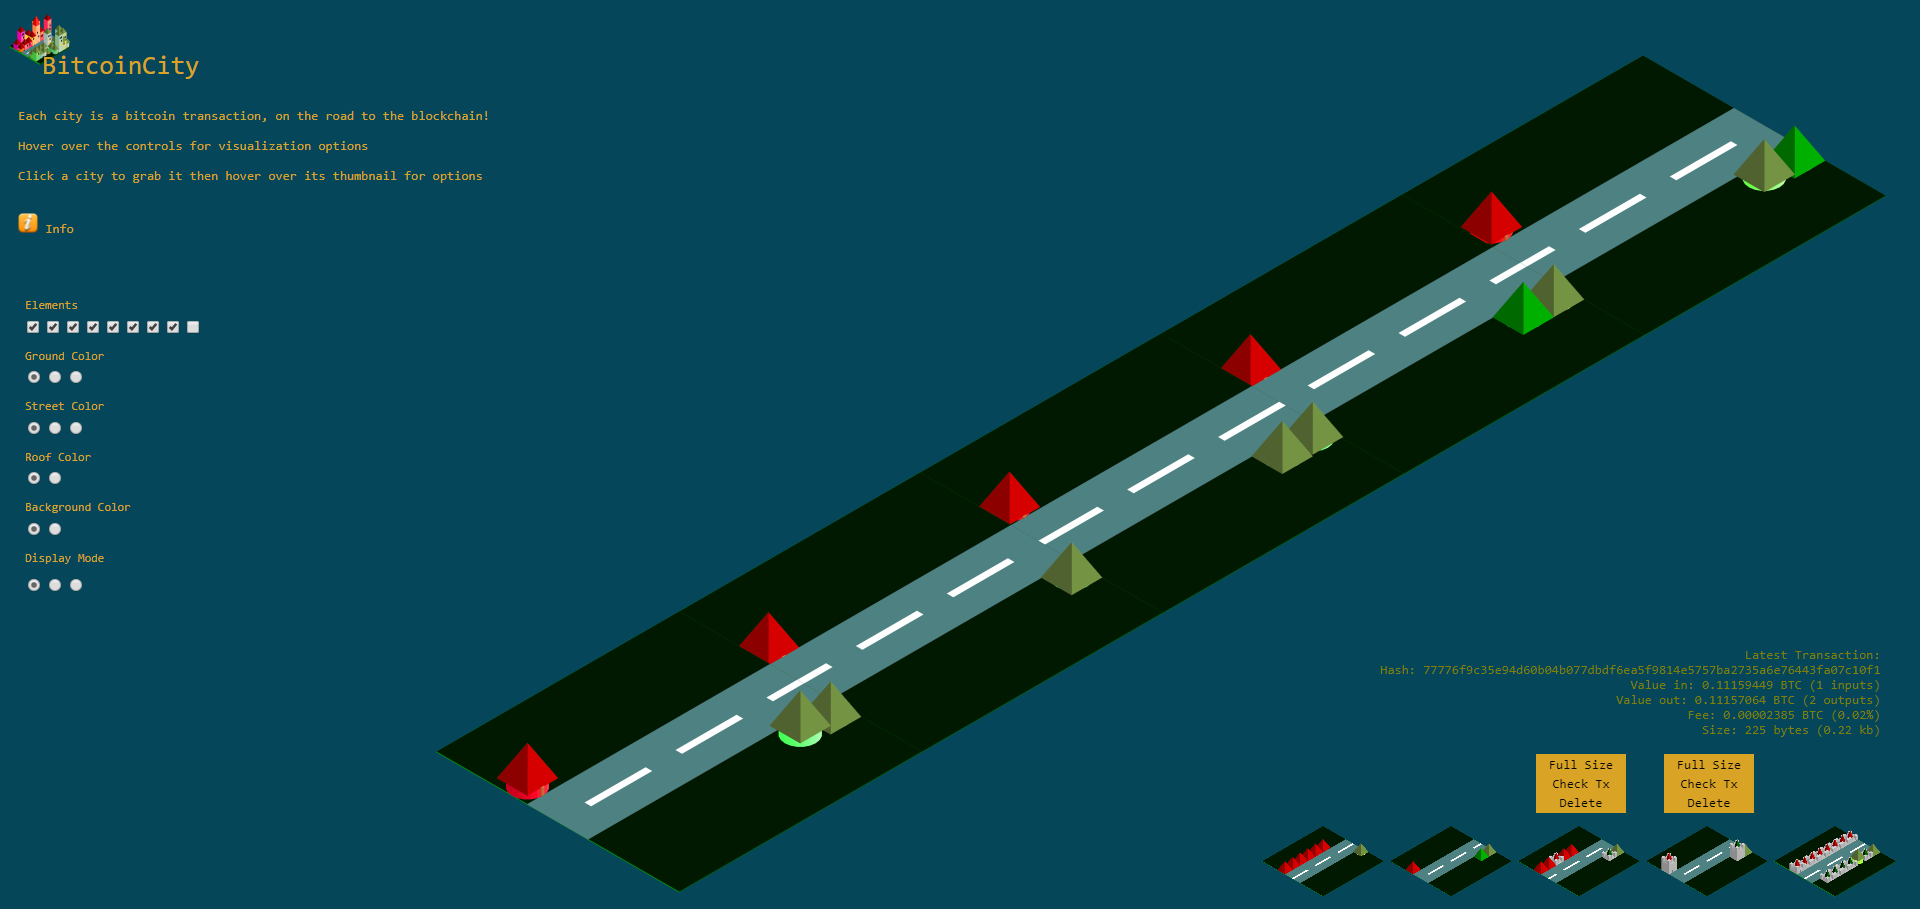
\includegraphics[width=\textwidth]{related_bitcoincity}
            \caption{BitcoinCity.}
            \label{fig:bitcoincity}
        \end{figure}
    \item \textbf{Blockseer} \cite{blockseer} \\
        Blockseer visualized the detailed information of accounts, transactions or blocks with tree structures. (Figure \ref{fig:blockseer})
        \begin{figure}[htb]
            \centering
            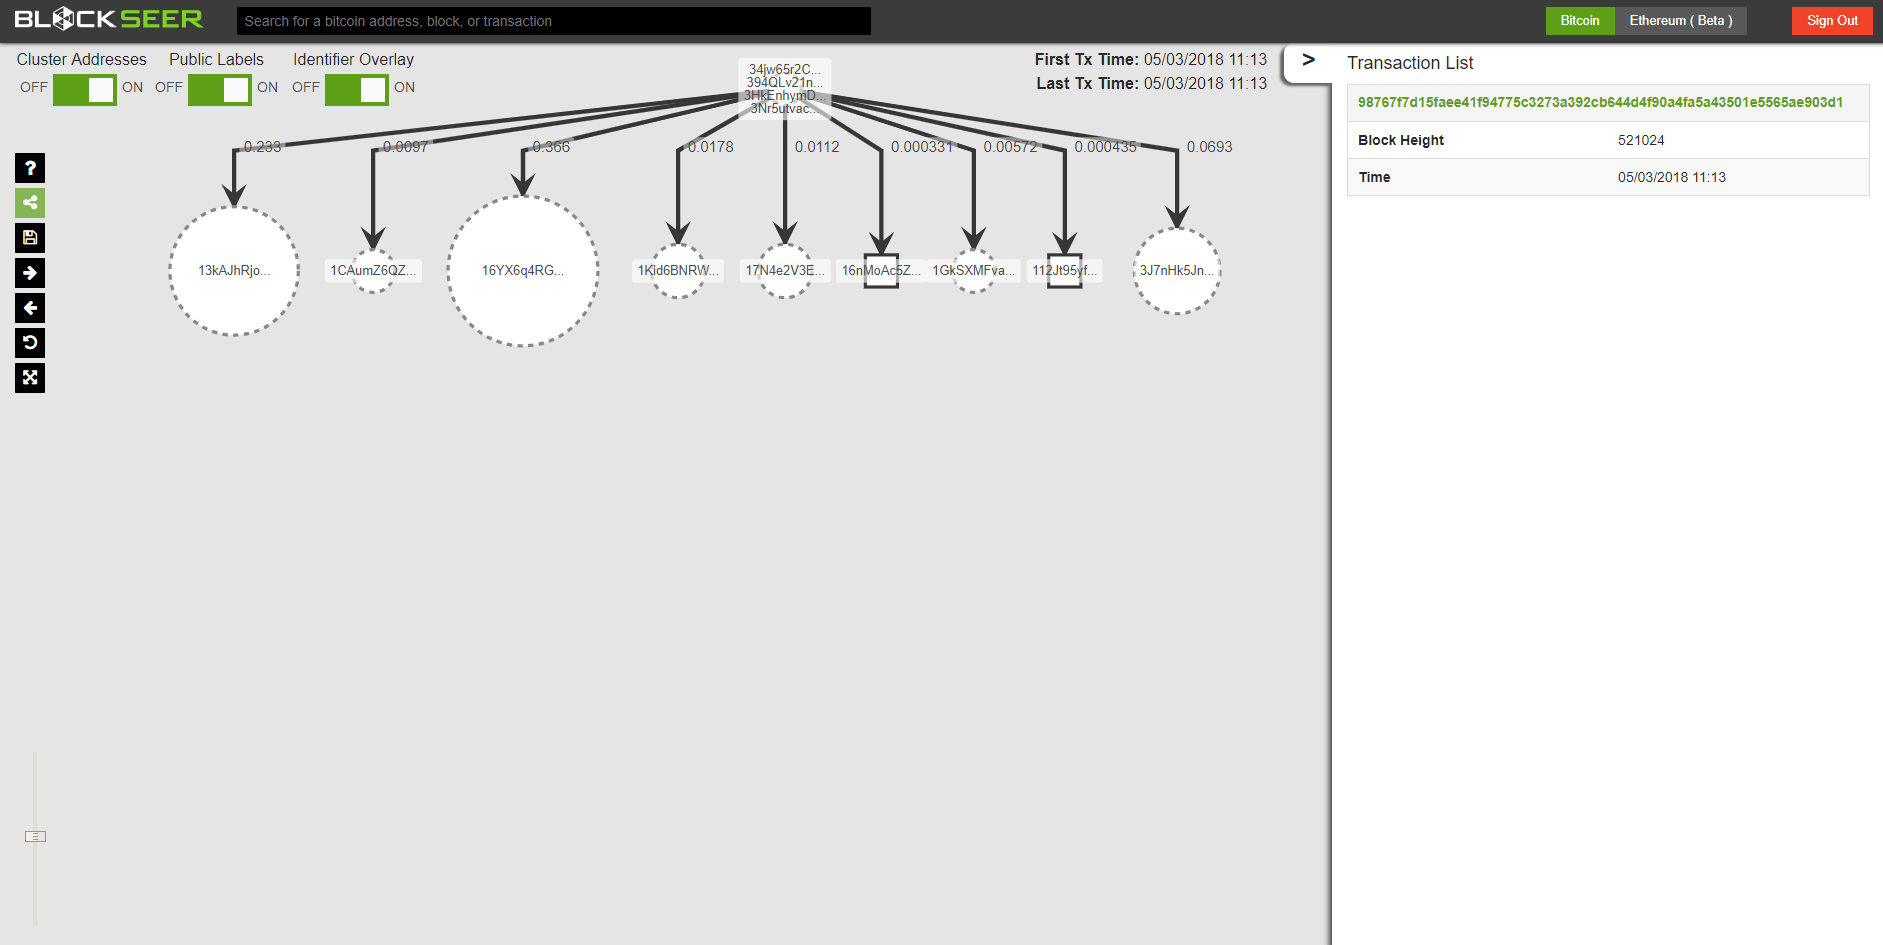
\includegraphics[width=\textwidth]{related_blockseer}
            \caption{Blockseer.}
            \label{fig:blockseer}
        \end{figure}
    \vspace*{\fill}
    \clearpage
    \vspace*{\fill}
    \item \textbf{DailyBlockchain} \cite{dailyblockchain} \\
        DailyBlockchain  displayed the spread of dynamic and live Bitcoin network. (Figure \ref{fig:dailyblockchain})
        \begin{figure}[htb]
            \centering
            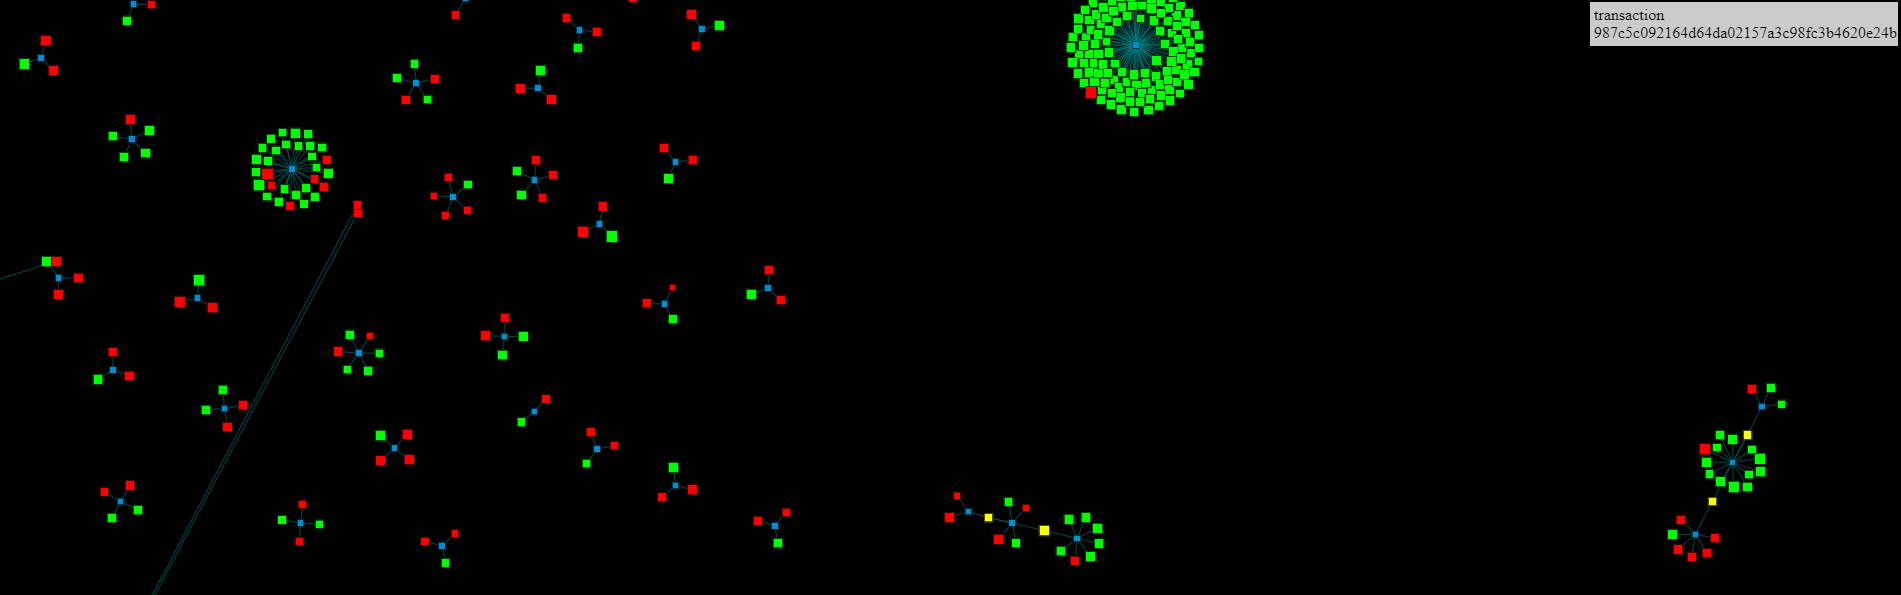
\includegraphics[width=\textwidth]{related_dailyblockchain}
            \caption{DailyBlockchain.}
            \label{fig:dailyblockchain}
        \end{figure}
    \item \textbf{Elliptic} \cite{elliptic} \\
        Elliptic visualized the whole history of Bitcoin like the Big Bang of the universe. (Figure \ref{fig:elliptic})
        \begin{figure}[htb]
            \centering
            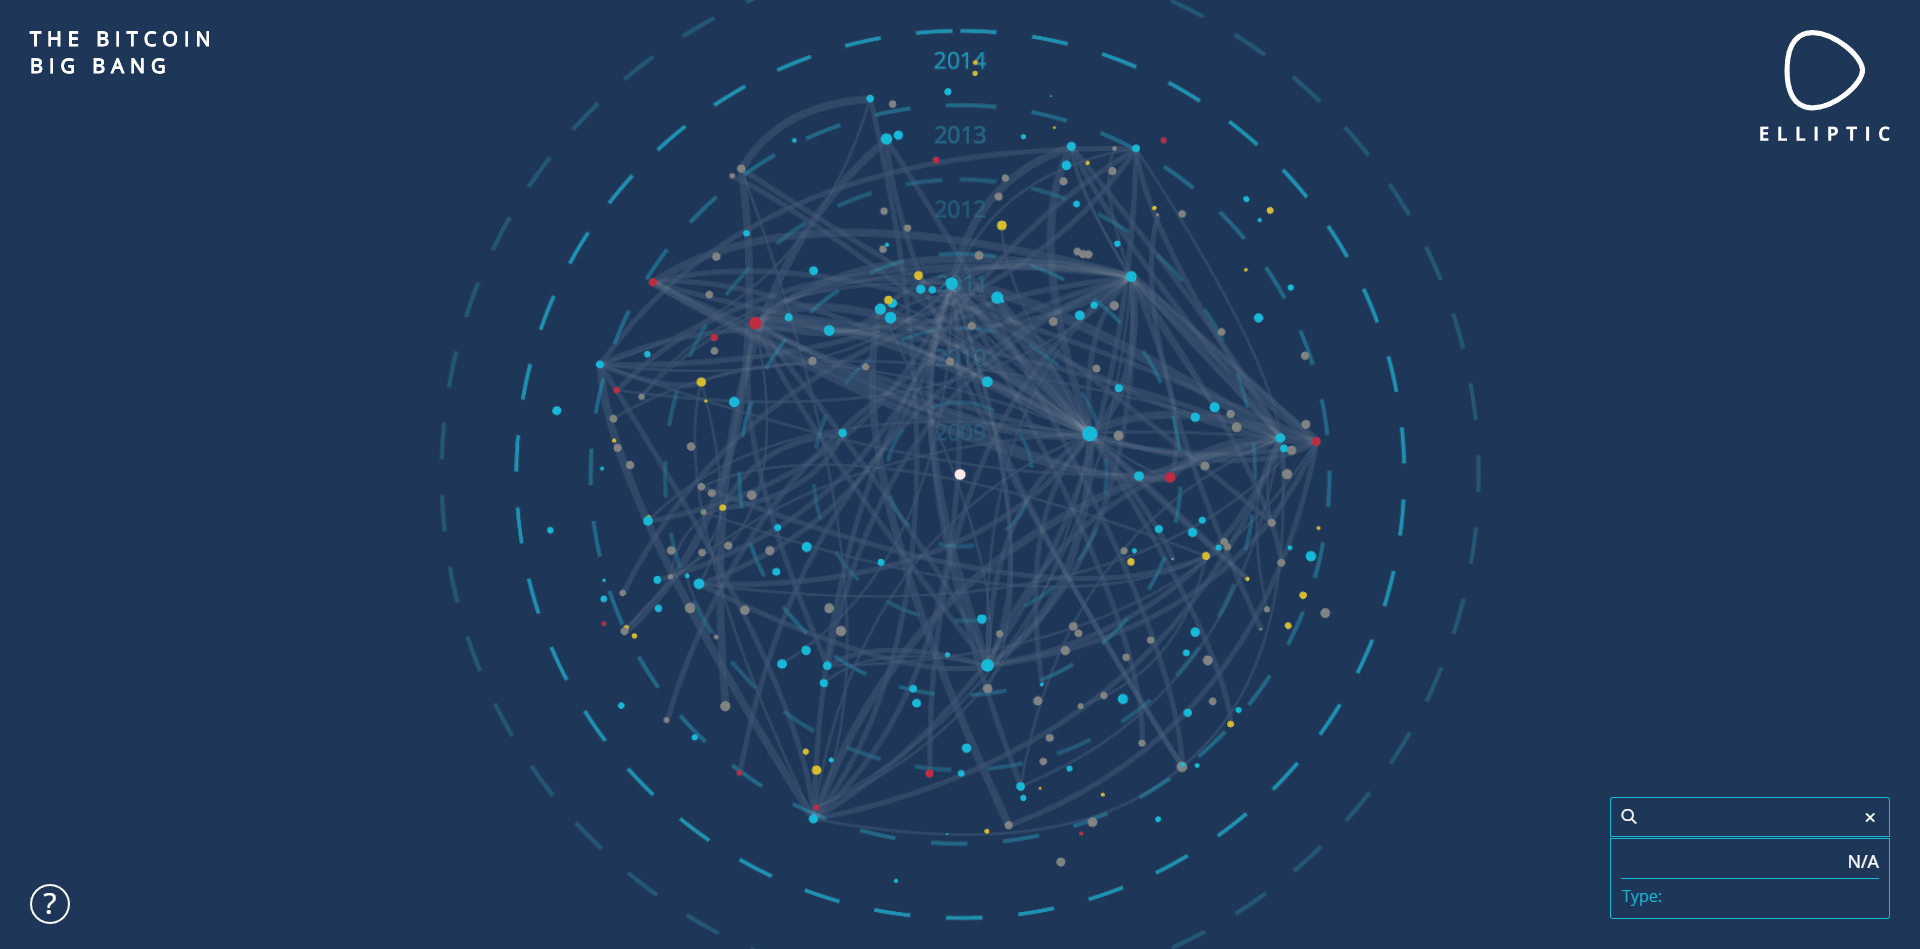
\includegraphics[width=\textwidth]{related_elliptic}
            \caption{Elliptic.}
            \label{fig:elliptic}
        \end{figure}
    \vspace*{\fill}
    \clearpage
    \item \textbf{Interaqt} \cite{interaqt} \\
        Interaqt rendered the Bitcoin transactions as circles. (Figure \ref{fig:interaqt})
        \begin{figure}[htb]
            \centering
            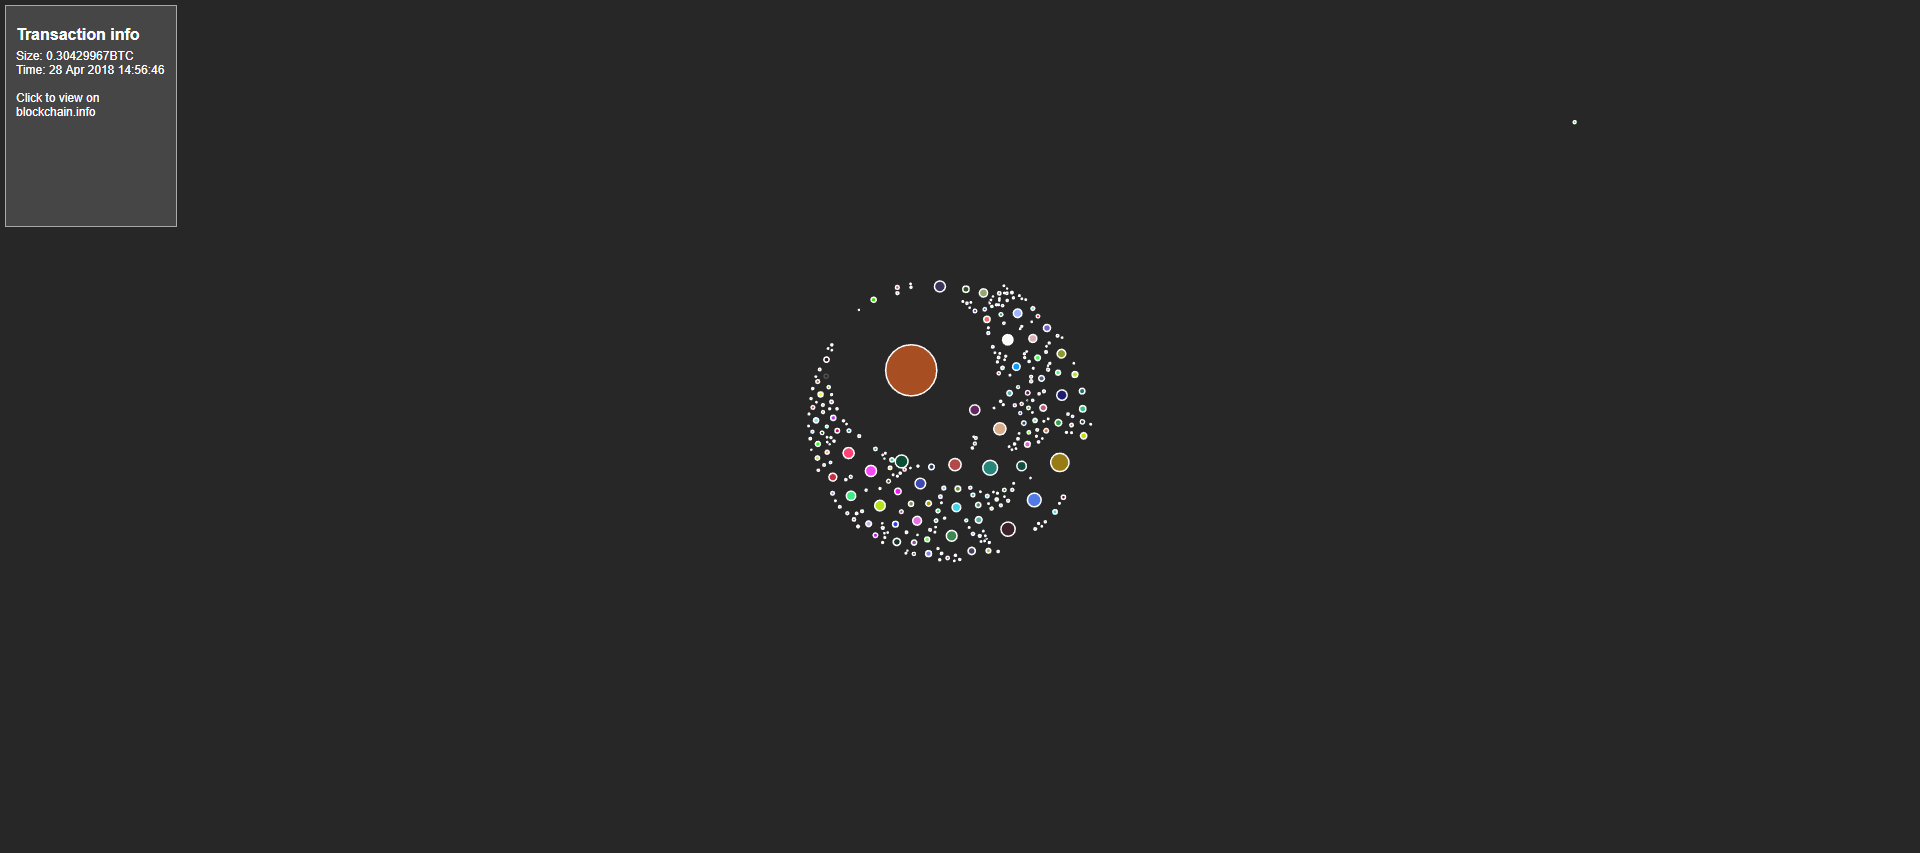
\includegraphics[width=\textwidth]{related_interaqt}
            \caption{Interaqt.}
            \label{fig:interaqt}
        \end{figure}
    \item \textbf{Live Globe} \cite{liveglobe} \\
        Live Globe combined the geographies of blocks and the earth together in the visualization. (Figure \ref{fig:live globe})
        \begin{figure}[htb]
            \centering
            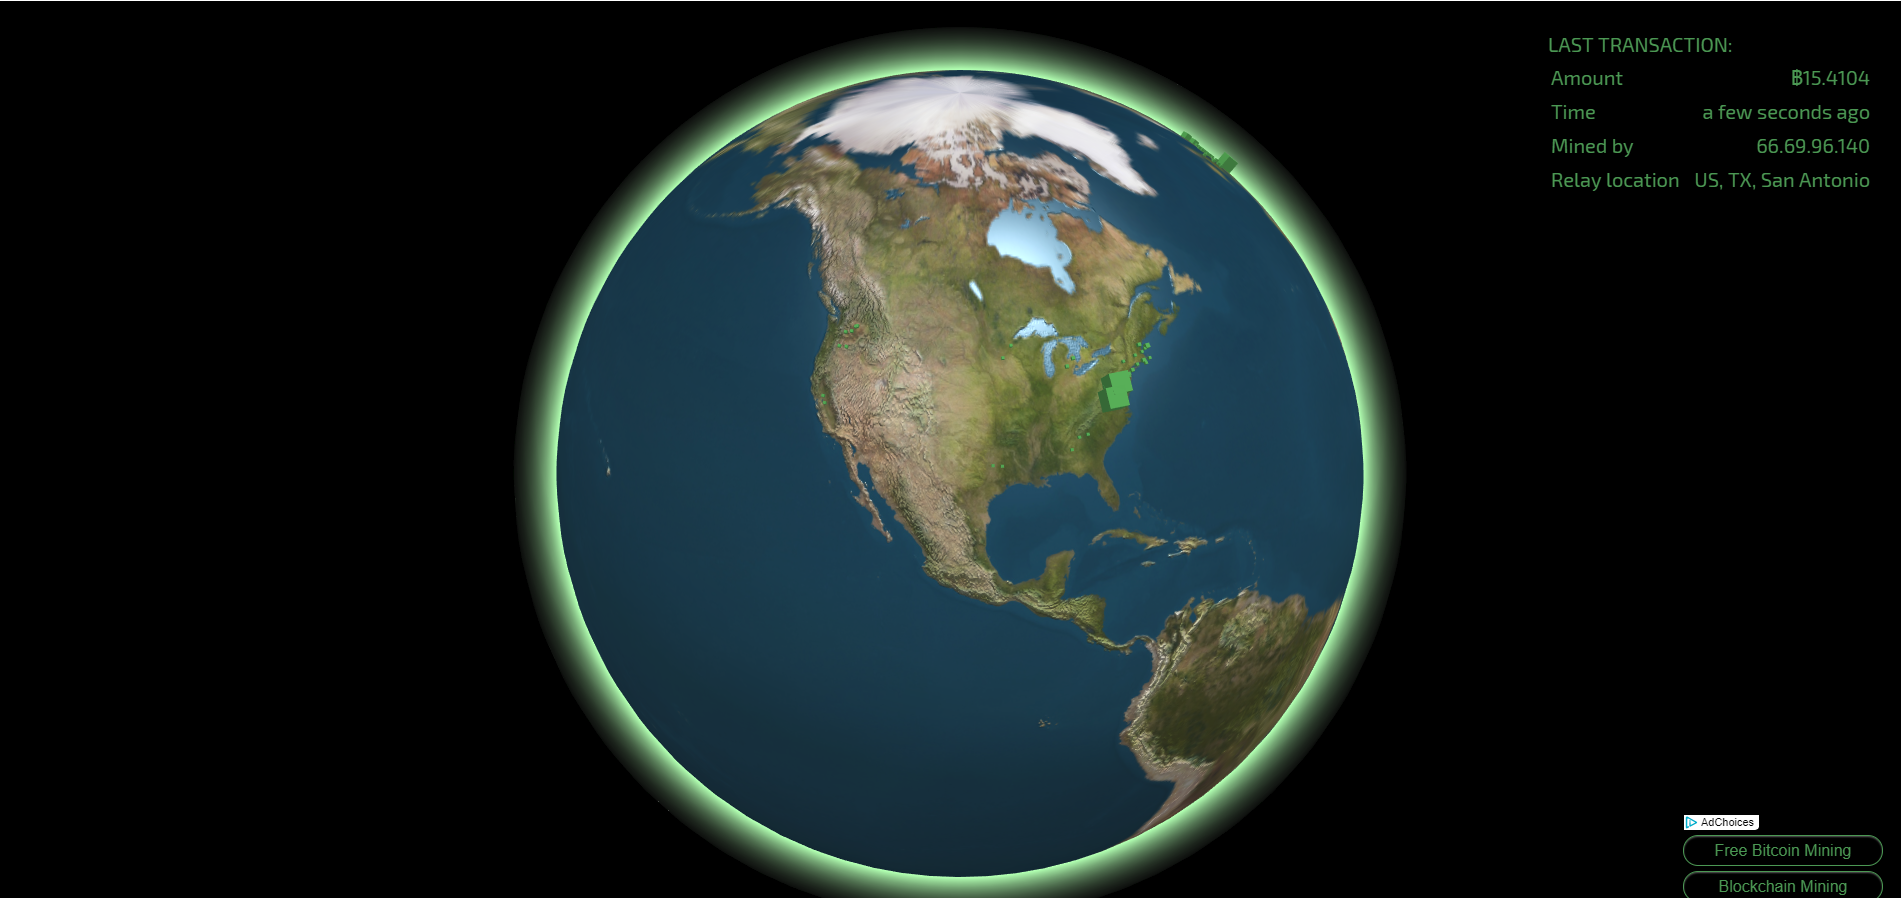
\includegraphics[width=\textwidth]{related_liveglobe}
            \caption{Live Globe.}
            \label{fig:live globe}
        \end{figure}
\end{itemize}

In addition to the 2D and 3D animations of the visualization of Bitcoin, there are applications which use tabular methods as the presentation of blockchains. Blockchain \cite{blockchain} and Etherscan \cite{etherscan} displayed the information of transactions and blocks in detail on Bitcoin and Ethereum networks. The results of them are demonstrated in Figure \ref{fig:tabular visualization}.

\begin{figure}[htb]
    \centering
    \begin{subfigure}[b]{1\textwidth}
        \centering
        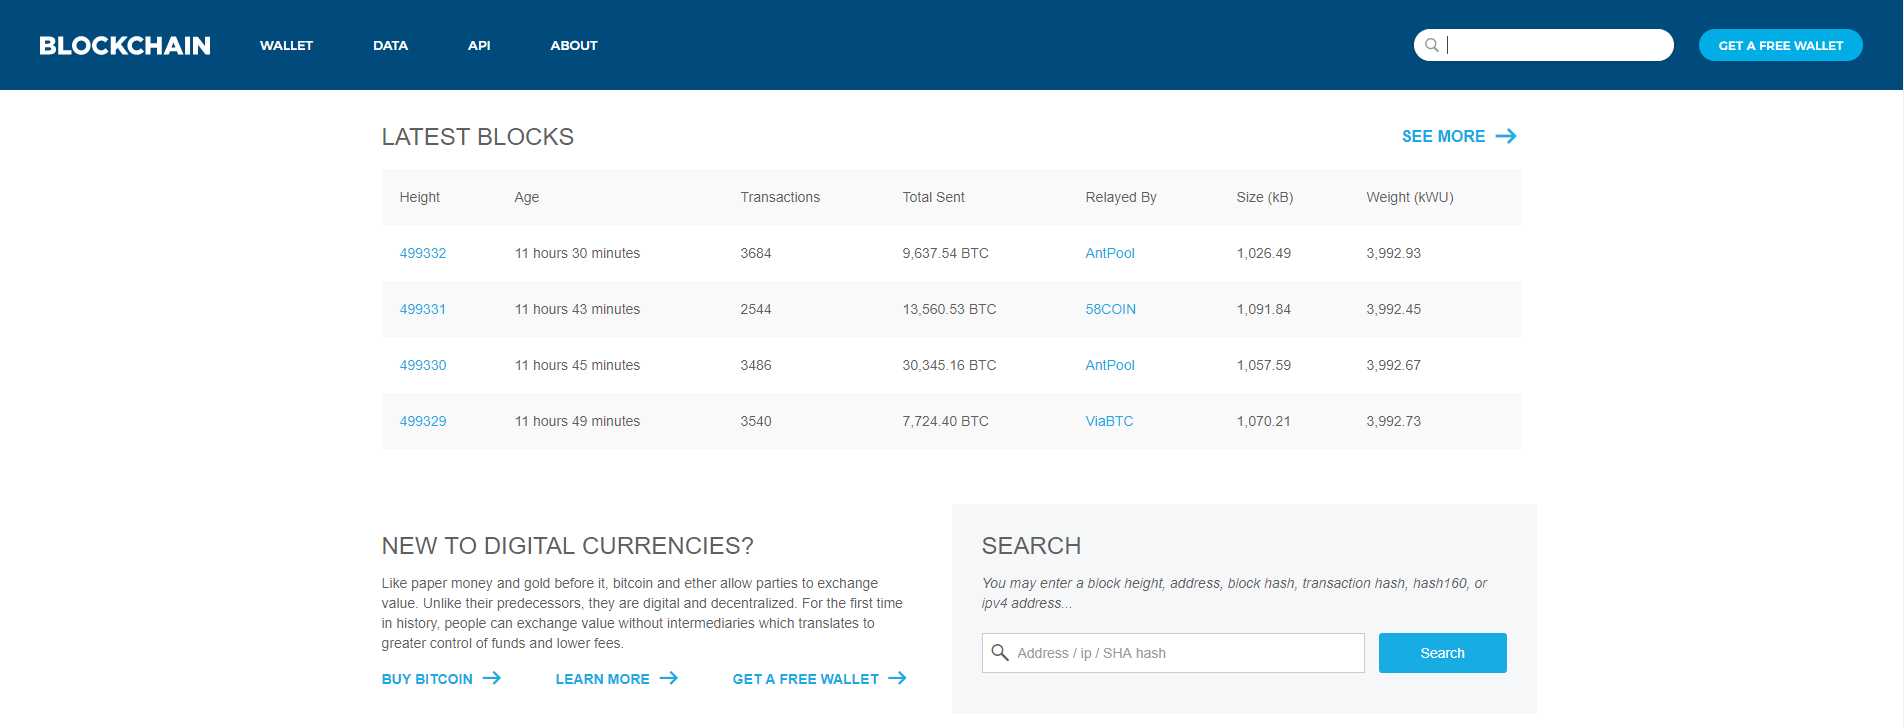
\includegraphics[width=\textwidth]{related_blockchain}
        \caption{Blockchain}
    \end{subfigure}

    \begin{subfigure}[b]{1\textwidth}
        \centering
        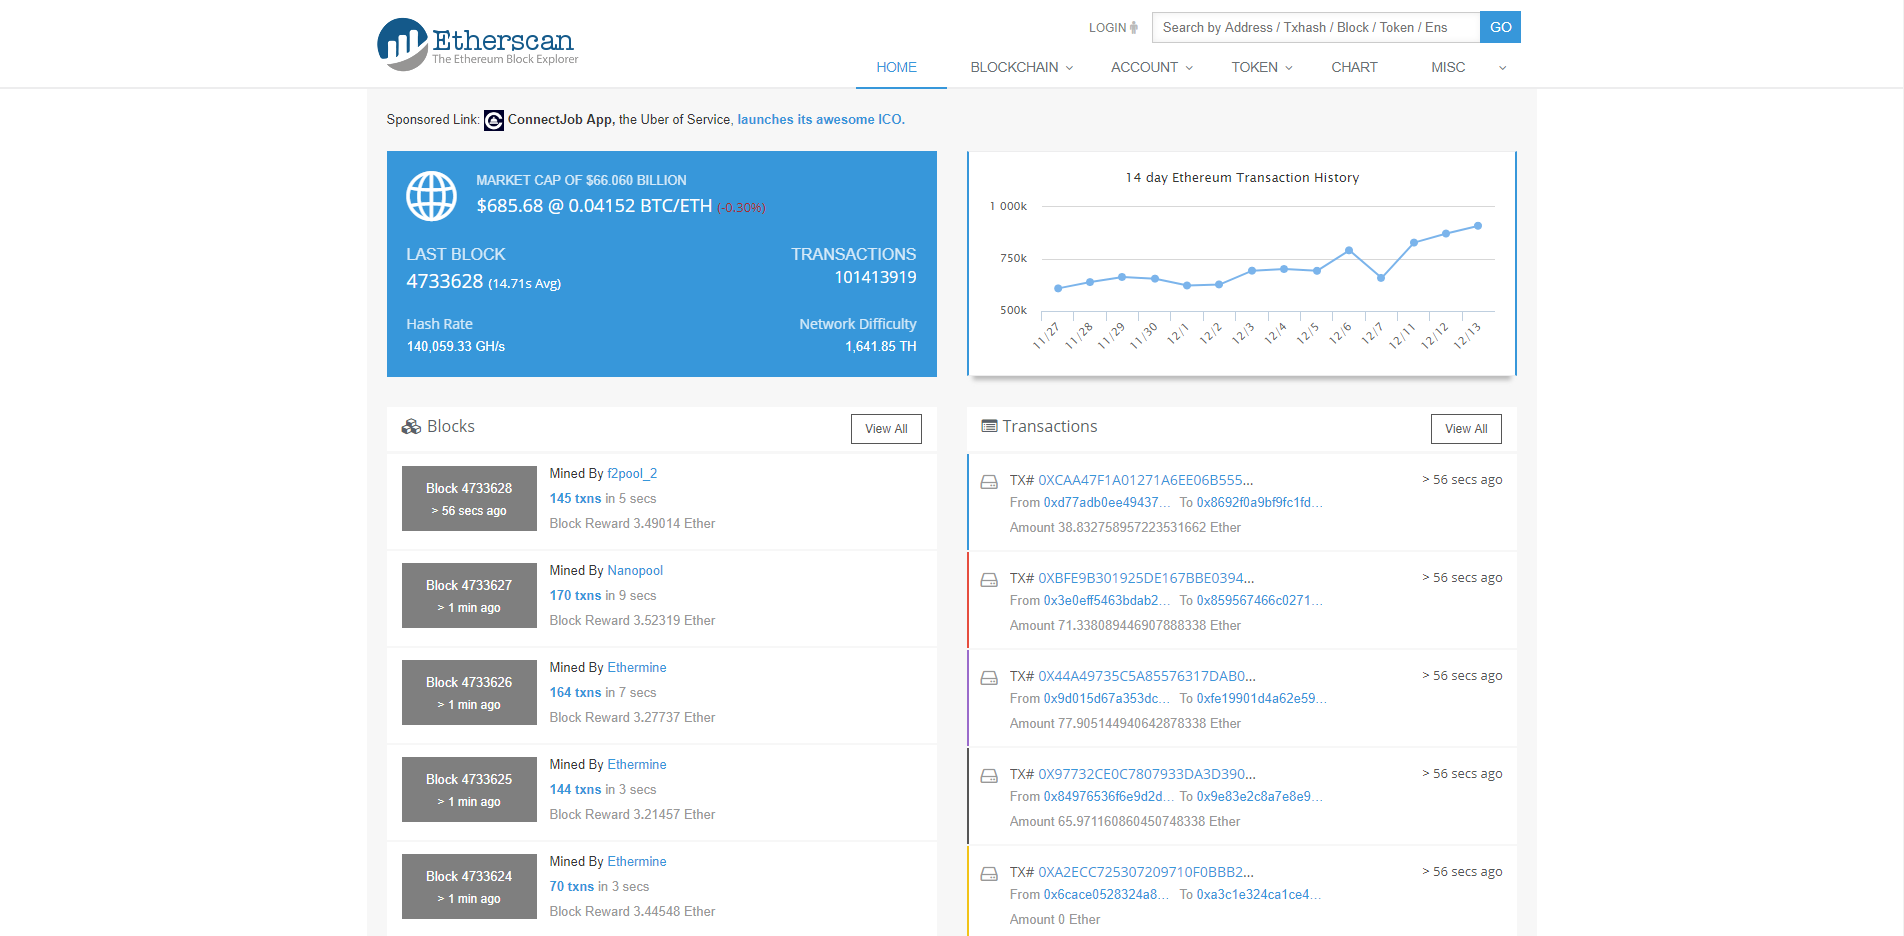
\includegraphics[width=\textwidth]{related_etherscan}
        \caption{Etherscan}
    \end{subfigure}

    \caption{Tabular Visualization.}
    \label{fig:tabular visualization}
\end{figure}

In short conclusion, although the above tools and applications showed amazing visualization methods of blockchains, their goals were to provide the static information and statistics instead of the dynamic mining processes that happened in a blockchain system. It is difficult to gain valuable understandings about the complex and dynamic mining processes in these applications.

\section{Analysis of Bitcoin Transactions}

As Bitcoin is the most popular and famous blockchain network currently, it is worth to explore the patterns of transactions and blocks to prevent malicious abuse of blockchain services. The nodes and transactions are anonymous on blockchain networks, so the recognition of patterns can be challengeable. Here we present some analysis methods and visualization technologies that can identify the relationships between nodes and transactions in time series on Bitcoin network.

\begin{itemize}
    \item \textbf{BitConeView: Visualization of Flows in the Bitcoin Transaction Graph} \cite{Battista2015} \\
        Giuseppe Di Battista et al. provided a visualization tool called \textit{BitConeView} that analyzed the flows of bitcoins in the transactions by timestamps. It can be used to analyze the patterns of the flows of bitcoins and locate tainted transactions.
    \item \textbf{Blockchain Explorer: An Analytical Process and Investigation Environment for Bitcoin} \cite{Kuzuno2017} \\
        To prevent the criminal activities and illegal behaviors that abuse the services of Bitcoin, Hiroki Kuzuno et al. proposed an analyzing system which managed the data and statistics of blockchains for the usages of law enforcement investigation and training.
    \item \textbf{Visualizing Dynamic Bitcoin Transaction Patterns} \cite{McGinn2016} \\
        Dan McGinn et al. focused on visualizing transactions of Bitcoin from the top-down viewpoint. The visualization of the large scale of data provided domain experts and the general public a tool to analyze and identify the transaction patterns with big data visualization methods.
    \item \textbf{Bitcoin Visualization} \cite{Saublet2015} \\
        The visual analytics tool that was proposed by Loïs Saublet enabled economists to analyze the metrics and actors on Bitcoin network and provided good user experience by working together with end users.
    \item \textbf{Bitcoin Transaction Graph Analysis} \cite{Fleder2015} \\
        Michael Fleder et al. proposed a graph-analysis framework that could analyze the relationships between public addresses and transactions. It can be used to match candidate Bitcoin transactions with the transactions in the reality. As a result, it demonstrated that the transactions are not entirely anonymous on Bitcoin network.
    \item \textbf{Exploring the Bitcoin Network} \cite{Baumann2014} \\
        The method proposed by Annika Baumann et al. employed graph mining algorithms to analyze the relationship of network usage and exchange rate. It served as the basis for the analysis of the anonymity and economic relationships on Bitcoin network.
\end{itemize}

In summary, the goals of the above tools and methods were to analyze the patterns and relationships of transactions and blocks. That is, they try to recognize patterns to prevent criminal activities and obtain economic inspiration. Therefore, The visualization results of the above literature served as bases and presentations for the analysis instead of the mining processes.

\section{Analysis of Consensus Protocols}

To analyze the network conditions of the proof-of-work based blockchain system, Amitai Porat et al. \cite{Porat} provided an application that was based on Ethereum platform. It simulated the asynchronous mining activities and network latency, and provided a real-time analysis of the blockchain system. They presented the potential applications of the blockchain technology through the analysis.

The main difference to our work is that we assume that miners have individual mining strategies instead of solving the same puzzles asynchronously. Therefore, there are miners who are able to solve the puzzles faster than the others under the same computing power, but they may suffer lower mining rewards. The combination of different mining strategies and the network delay makes the visualization of the blockchain system dynamic and undetermined. Thus our solution is suitable for researchers to find the influences of different factors on the blockchain system. Moreover, their work focused on finding the potential applications of Ethereum platform. On the other hand, our work emphasize on visualizing the continuous mining processes while miners have different mining strategies and suffer from the network delay. 

\section{Our Approach}

To focus on the dynamic mining activities, our tool provides a real-time visualization of the mining processes that cannot be achieved by the above visualization tools and applications. Through our visualization, users can observe the mining processes step by step. Moreover, our visualization is independent of specific blockchain platforms, e.g., Bitcoin and Ethereum, because we built a simple simulation of the blockchain system by ourselves. Therefore, we can concentrate on the mining processes which is the most important activities in a proof-of-work based blockchain system.

\begin{figure}[htb]
    \centering
    \begin{subfigure}[b]{1\textwidth}
        \centering
        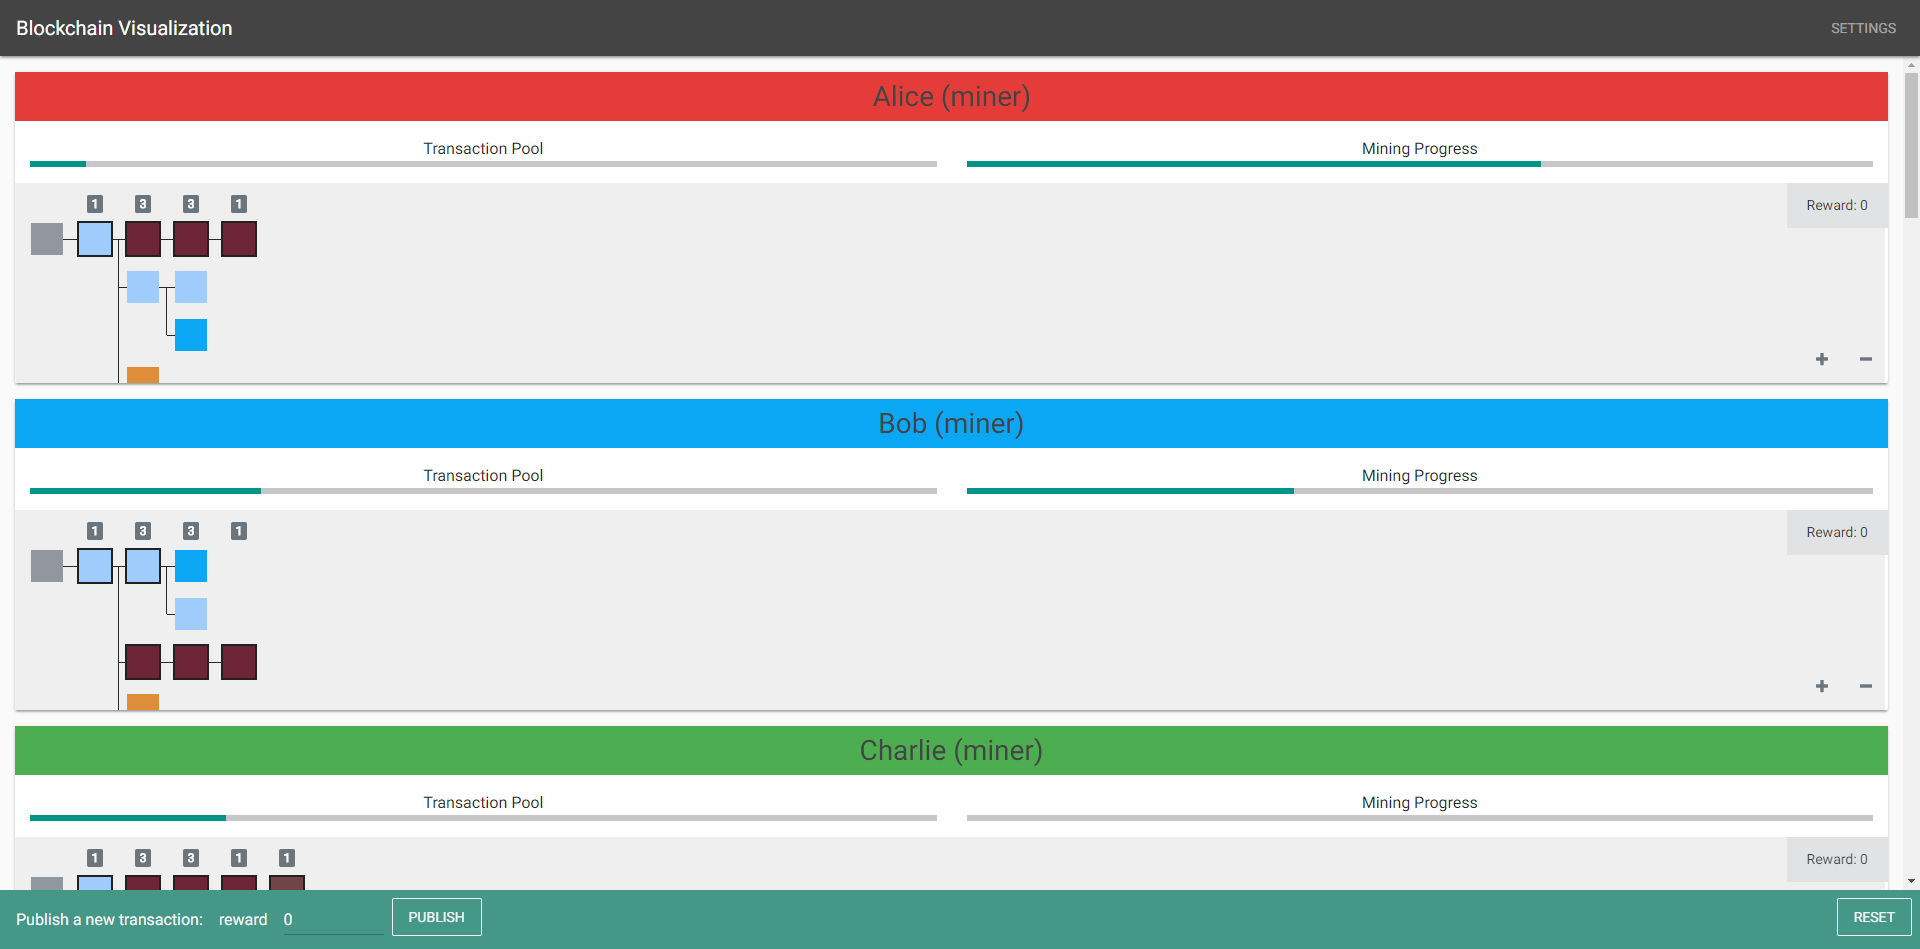
\includegraphics[width=\textwidth]{related_us1}
        \caption{Mining Step 1}
    \end{subfigure}

    \begin{subfigure}[b]{1\textwidth}
        \centering
        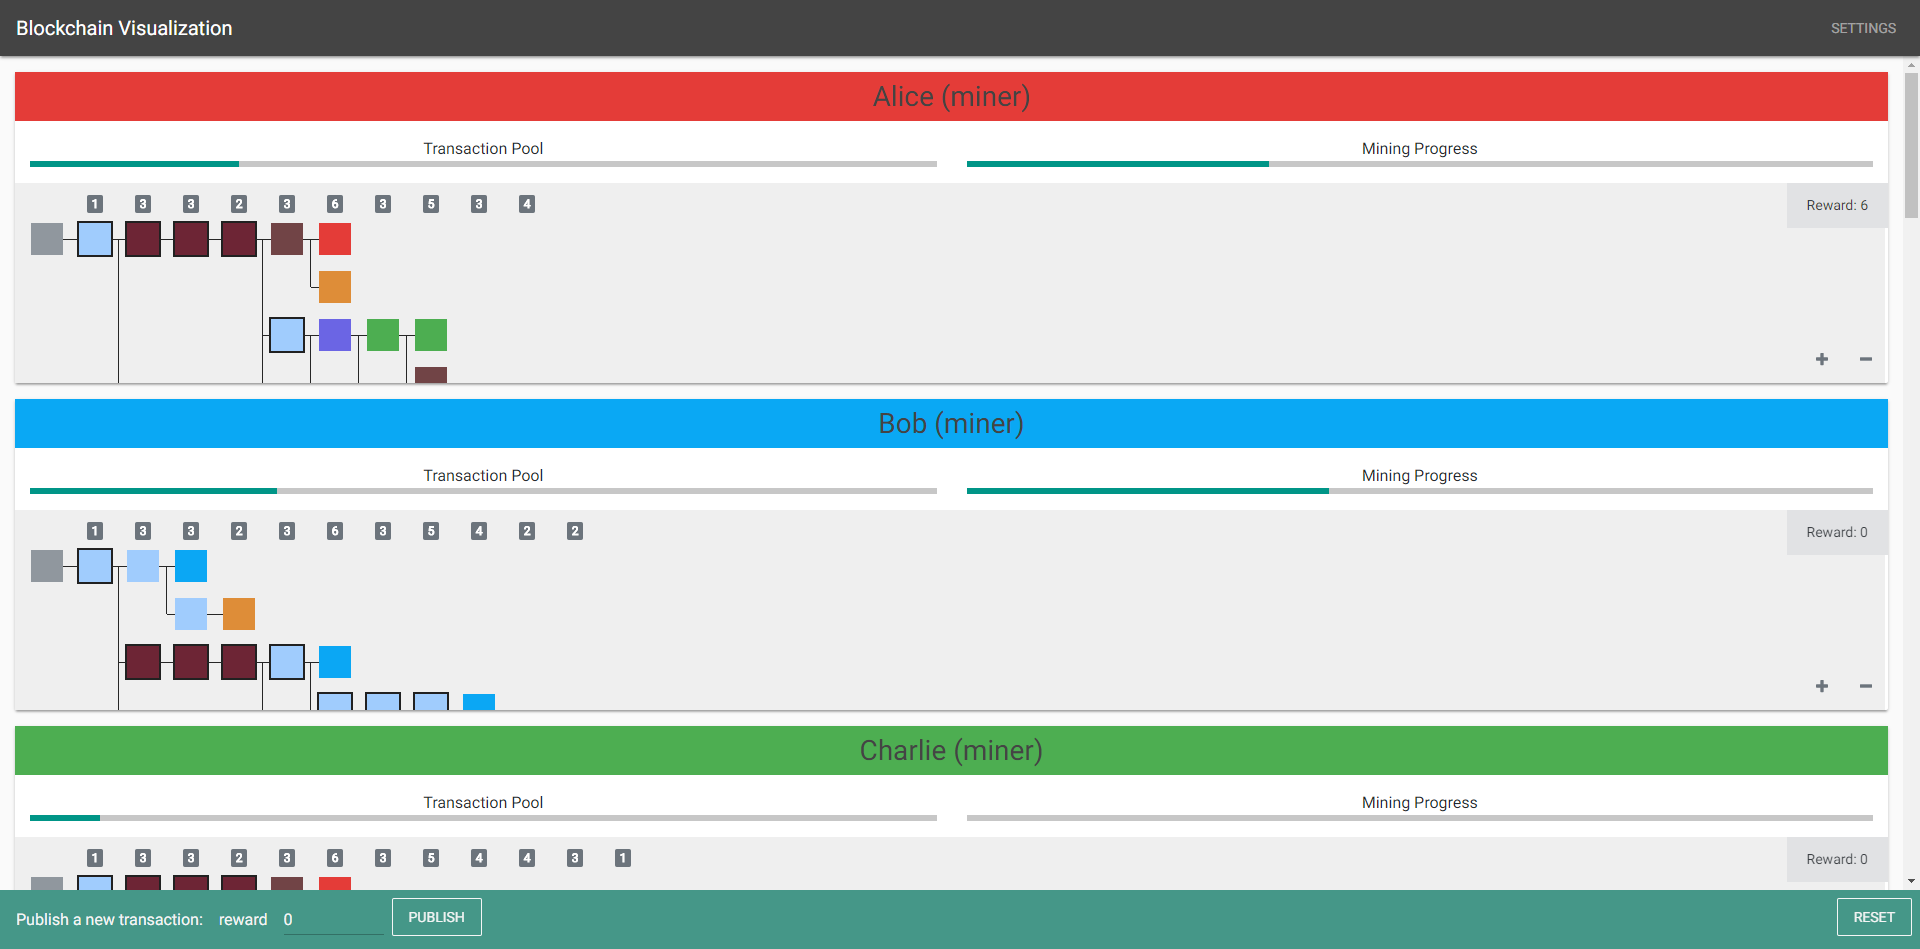
\includegraphics[width=\textwidth]{related_us2}
        \caption{Mining Step 2}
    \end{subfigure}

    \caption{Steps of Mining.}
    \label{fig:steps of mining}
\end{figure}

As we can see in Figure \ref{fig:steps of mining}, the tree structures of the blockchain keep growing while the mining activities continue. The basic visualization ideas of our project are inspired by a former project called “Kooperative Music Box” \cite{musicbox} which was developed by Fraunhofer Blockchain-Labor. It used shapes and colors to distinguish different blocks and transactions which were generated by different nodes. As a result, in the visualization application, the blocks are represented as squares, and they are chained by lines to form tree structures, and the colorful blocks are generated by different miners.

Our project aims to visualize all the dynamic mining processes that could happen in a blockchain system, with the factors of the network delay and the different mining strategies. This distinguishes our work to all the related works mentioned before. Consequently, our work is worthwhile as a contribution and a trial to the blockchain research area.
